Se realizó el experimento a un total de 36 sujetos, de forma que se tuviera una muestra de tamaño $n=12$ para cada instrumento. Todos los sujetos son personas jóvenes en el rango de edad de 18-30 años, escogidos aleatoriamente (mediante un script de Python). Las pruebas fueron realizadas en la tarde (3pm-6pm), el mismo día:

\begin{table}[H]
    \begin{center}
        \begin{tabular}{|c |p{2.5cm} |p{2.5cm} |p{3cm}|c|}
            \hline
            \textbf{Nombre} & {\textbf{Dopamina pre-Instrumento}} & {\textbf{Dopamina post-Instrumento}} & {\textbf{Aumentos o Disminuciones}} & \textbf{Instrumento} \\
            \hline
            Abigail Collins & 19.6 & 19.1 & -0.5 & PIANO \\
            Abigail Sato & 18.2 & 18.1 & -0.1 & PIANO \\
            Alfred Bauer & 20.4 & 20.5 & 0.1 & PIANO \\
            Alina Bager & 18.2 & 18.5 & 0.3 & PIANO \\
            Andrej Grimm & 22.5 & 22.9 & 0.4 & PIANO \\
            Conor Kimura & 21.7 & 22.9 & 1.2 & PIANO \\
            Corina Page & 20.6 & 20.2 & -0.4 & PIANO \\
            Daichi Wilson & 20.3 & 20.1 & -0.2 & PIANO \\
            Daiki Regan & 17.8 & 17.1 & -0.7 & PIANO \\
            Dane Sorensen & 18.9 & 18.9 & 0 & PIANO \\
            Dr David Solberg & 20.3 & 19.7 & -0.6 & PIANO \\
            Dieter Walther & 16.1 & 15.6 & -0.5 & PIANO \\
            Jorn Blomgren & 18.7 & 19.3 & 0.6 & FLAUTA \\
            Sophie Wilson & 22.1 & 22.1 & 0 & FLAUTA \\
            Riku McCarthy & 21 & 21.3 & 0.3 & FLAUTA \\
            Ethan Connolly & 17.3 & 17.2 & -0.1 & FLAUTA \\
            Sorena Lund & 22.1 & 22.7 & 0.6 & FLAUTA \\
            Raum Carlsen & 21.2 & 21.3 & 0.1 & FLAUTA \\
            Dylan Regan & 17.8 & 17.9 & 0.1 & FLAUTA \\
            Anke Jaeger & 21.4 & 21.4 & 0 & FLAUTA \\
            Ren Edwards & 18.7 & 17.8 & -0.9 & FLAUTA \\
            Erin Morris & 22 & 21.5 & -0.5 & FLAUTA \\
            Ursula Carlsen & 20.6 & 20.9 & 0.3 & FLAUTA \\
            Arvid Solberg & 20.8 & 21.5 & 0.7 & FLAUTA \\
            Christian Carlsen & 20.6 & 20.3 & -0.3 & CELLO \\
            Amber Edwards & 25.4 & 25 & -0.4 & CELLO \\
            Gala Thorn & 20.3 & 20.8 & 0.5 & CELLO \\
            Sonja Bager & 20.4 & 20.7 & 0.3 & CELLO \\
            Nanako Morris & 19.7 & 20 & 0.3 & CELLO \\
            Valdemar Eklund & 20.2 & 20.1 & -0.1 & CELLO \\
            Kornelia Moser & 21.2 & 21.4 & 0.2 & CELLO \\
            Lars Sorensen & 20.4 & 20.8 & 0.4 & CELLO \\
            Leonie Thorn & 17.3 & 17.5 & 0.2 & CELLO \\
            Liam Moore & 15.9 & 16.3 & 0.4 & CELLO \\
            Malena Landvik & 18.4 & 19.3 & 0.9 & CELLO \\
            Marc Dietrich & 17.8 & 17.8 & 0 & CELLO \\
            \hline
        \end{tabular}
        \caption{Base de datos de las pruebas realizadas}
    \end{center}
\end{table}


Considerando el objetivo de la investigación, se consideró óptimo utilizar las diferencias obtenidas de niveles de dopamina en la orina antes y después de tocar el instrumento asignado:

\begin{table}[H]
    \begin{center}
        \begin{tabular}{ |ccc| }
            \hline
                \textbf{PIANO} & \textbf{CELLO} & \textbf{FLAUTA} \\
            \hline
                0.5 & 0.3 & 0.6 \\
                0.1 & 0.4 & 0.1 \\
                -0.1 & 0.5 & 0.1 \\
                -0.3 & 0.3 & 0 \\
                -0.4 & 0.3 & -0.9 \\
                1.2 & -0.1 & -0.5 \\
                -0.4 & 0.2 & 0.3 \\
                -0.2 & 0.4 & 0.7 \\
                -0.7 & 0.2 & 0.6 \\
                0 & 0.4 & 0 \\
                -0.6 & 0.9 & 0.3 \\
                -0.5 & 0 & -0.1 \\
            \hline
        \end{tabular}
        \caption{Muestras utilizadas en el estadístico de prueba para cada instrumento. }
    \end{center}
\end{table}


%----------------------------------------------------------------------------------------
*Los datos de las muestras previamente mostradas, fueron analizadas de forma gráfica: 
\subsection{Histogramas}
\begin{center}
    \begin{figure}[H]
        \centering
        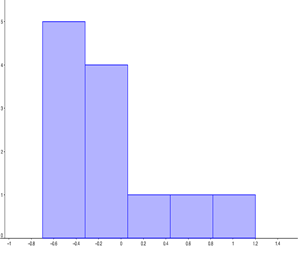
\includegraphics[width=0.3\textwidth]{./appendages/HP.png}
        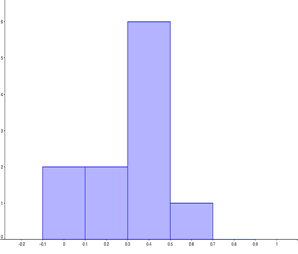
\includegraphics[width=0.3\textwidth]{./appendages/HC.png}
        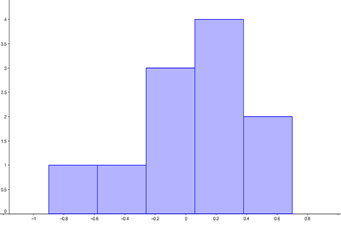
\includegraphics[width=0.3\textwidth]{./appendages/HF.png}
        \caption{Histogramas de piano, cello y flauta respectivamente. *Realizado en Geogebra.}
    \end{figure}
\end{center}
Los histogramas nos demuestran de forma gráfica que todas las muestras tienen distribuciones de frecuencias distintas.

%----------------------------------------------------------------------------------------
\subsection{Diagrama de caja y bigotes}
\begin{center}
    \begin{figure}[H]
        \centering
        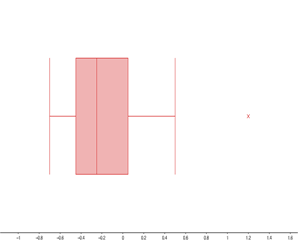
\includegraphics[width=0.3\textwidth]{./appendages/DBP.png}
        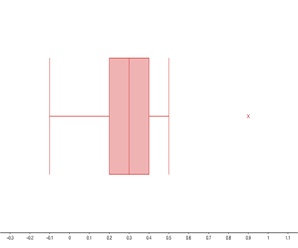
\includegraphics[width=0.3\textwidth]{./appendages/DBC.png}
        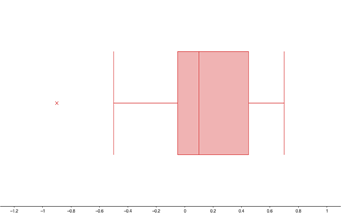
\includegraphics[width=0.3\textwidth]{./appendages/DBF.png}
        \caption{Diagrama de Caja y Bigotes de piano, cello y flauta respectivamente. *Realizado en Geogebra.}
    \end{figure}
\end{center}
El diagrama de caja es un método estandarizado para representar gráficamente una serie de datos numéricos a través de sus cuartiles. El diagrama es diferente para las tres muestras, con distinta variabilidad fuera de los cuartiles superior e inferior.

%----------------------------------------------------------------------------------------
\subsection{Normalidad}
\begin{center}
    \begin{figure}[H]
        \centering
        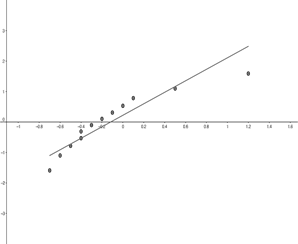
\includegraphics[width=0.3\textwidth]{./appendages/NP.png}
        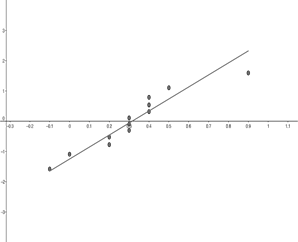
\includegraphics[width=0.3\textwidth]{./appendages/NC.png}
        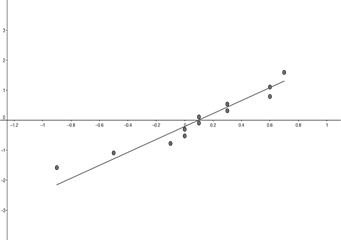
\includegraphics[width=0.3\textwidth]{./appendages/NF.png}
        \caption{Gráfica QQ de piano, cello y flauta respectivamente. *Realizado en Geogebra.}
    \end{figure}
\end{center}

Las muestras de las tres poblaciones no tienen normalidad. De esta forma, todas las pruebas que se podían realizar tenían que aceptar el supuesto de no normalidad. Por lo tanto, este proyecto de investigación utilizó únicamente pruebas de hipótesis no paramétricas.
